\chapter{Algorithme de Grover}
\label{appendix:grover}

\section{Rappels d'algèbre: projection et reflection}
On utilise ici la notation de Dirac pour noter les vecteurs, et on ne norme pas les vecteurs pour plus de simplicité dans les calculs. Les raisonnements restent les mêmes si on respectait la norme.

Soient deux vecteurs $\ket{u}$ et $\ket{v}$, avec $\ket{v}$ normalisé.

\begin{definition}
  La matrice de projection $P$ de $\ket{u}$ sur $\ket{v}$ est définie par $P = \ket{v} \cdot \bra{v}$.
\end{definition}

\begin{definition}
  La matrice de reflection $R$ de $\ket{u}$ par rapport à $\ket{v}$ est définie par $R = 2 \ket{v} \cdot \bra{v} - I$.
\end{definition}

\begin{ex}
Prenons $\ket{u}=\begin{bmatrix}2\\3\end{bmatrix}$ et $\ket{v}=\begin{bmatrix}1\\-2\end{bmatrix}$.

On projete $\ket{u}$ sur $\ket{v}$:

$P = \frac{\ket{v} \cdot \bra{v}}{\norm{v}^2} = \begin{bmatrix}\frac{1}{\sqrt{5}} & \frac{-2}{\sqrt{5}}\\\frac{-2}{\sqrt{5}} & \frac{4}{\sqrt{5}}\end{bmatrix}$
\medbreak
Soit: $\ket{u_v} = P\ket{u} = \begin{bmatrix}-0.8\\1.6\end{bmatrix}$
\end{ex}

\begin{ex}
Prenons à nouveau $\ket{u}=\begin{bmatrix}2\\3\end{bmatrix}$ et $\ket{v}=\begin{bmatrix}1\\-2\end{bmatrix}$.
On effectue une reflection de $\ket{u}$

$R = 2 \times \frac{\ket{v} \cdot \bra{v}}{\norm{v}^2} - I = 2 \times \begin{bmatrix}\frac{1}{\sqrt{5}} & \frac{-2}{\sqrt{5}}\\\frac{-2}{\sqrt{5}} & \frac{4}{\sqrt{5}}\end{bmatrix} - \begin{bmatrix}1 & 0 \\ 0 & 1\end{bmatrix}$
\end{ex}

La première étape est la double projection $2\times P$, ce qui donne le vecteur $\begin{bmatrix}-1.6\\3.2\end{bmatrix}$.

La deuxième étape est d'enlever le vecteur initial, ce qui donne le vecteur $\ket{u_R} = \begin{bmatrix}-3.6\\0.2\end{bmatrix}$.

On peut vérifier les angles $\theta_{UV}$ et $\theta_{VU_R}$:

$\theta_{UV} = \arccos({\frac{u \cdot v}{\norm{u}\norm{v}}}) = \arccos({\frac{-4}{\sqrt{13} \times \sqrt{5}}}) = 119.7\degree$

$\theta_{VU_R} = \arccos({\frac{v \cdot u_R}{\norm{v}\norm{u_R}}}) = \arccos({\frac{-4}{\sqrt{5} \times \sqrt{13}}}) = 119.7\degree$

Les deux angles sont bien égaux, on a effectué une reflection.

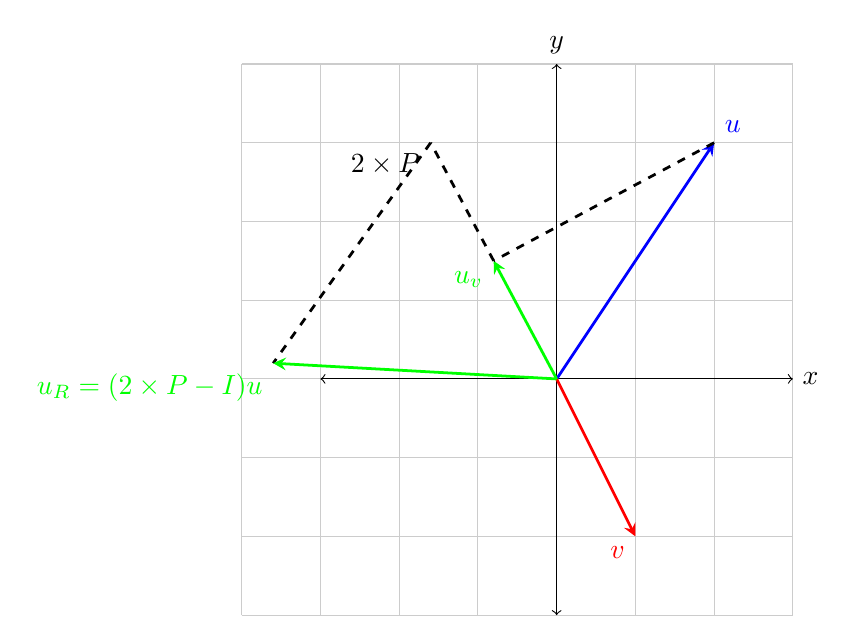
\begin{tikzpicture}
  \draw[thin,gray!40] (-4,-3) grid (3,4);
  \draw[<->] (-3,0)--(3,0) node[right]{$x$};
  \draw[<->] (0,-3)--(0,4) node[above]{$y$};
  \draw[line width=1pt,blue,-stealth](0,0)--(2, 3) node[anchor=south west]{$\boldsymbol{\ket{u}}$};
  \draw[line width=1pt,red,-stealth](0,0)--(1,-2) node[anchor=north east]{$\boldsymbol{\ket{v}}$};
  \draw[line width=1pt,green,-stealth](0,0)--(-0.8,1.5) node[anchor=north east]{$\boldsymbol{\ket{u_v}}$};
  \draw[line width=1pt,gray!200,dashed](2, 3) -- (-0.8,1.5){};
  \draw[line width=1pt,gray!200,dashed](-0.8,1.5)--(-1.6,3.0) node[anchor=north east]{$\boldsymbol{2 \times P}$};
  \draw[line width=1pt,gray!200,dashed](-1.6,3.0)--(-3.6,0.2) node[anchor=north east]{};
  \draw[line width=1pt,green,-stealth](0,0)--(-3.6,0.2) node[anchor=north east]{$\boldsymbol{\ket{u_R} = (2 \times P - I)\ket{u}}$};
\end{tikzpicture}

\section{Problème à résoudre}
Soit une base de données non triée à $N$ entrées. Nous voulons trouver un algorithme permettant de chercher efficacement un enregistrement dans cette base.

% \subsection{Principe de l'algorithme}
% L'algorithme de Grover permet de résoudre ce problème en quantique, en disposant de $N$ qubits intriqués pour calculer $2^N$ état 
% (donc si on a $N$ entrées dans la base, il nous faut $log_2(N)$ qubits intriqués). Dans le cas de cet algorithme, on considère le problème suivant:
% \medbreak
% On marque $\{0, 1, 2, ..., N-1\}$ les enregistrements de la base de données, et on dénote $\omega$ l'état inconnu recherché. On dispose de la fonction suivante:

% $f(x) = 
%  \begin{cases}
%    1, & \text{si x vérifie le critère} \; \omega \\
%    0, & \text{sinon}
%  \end{cases}
% $

% A la fin, on obtient un set de résultat. Or, lors de la mesure on va avoir au hasard une des solutions suivant les probabilités de chaque état, alors qu'on cherche
% juste à savoir la (ou les) bonnes solutions. On rajoute donc une amplification d'amplitude permettant d'augmenter les probabilités des bons résultats et de diminuer
% celles des mauvais.


\subsubsection*{Initialisation}

On commence avec :
$\ket{u_0} = (\ket{0}^{\bigotimes n}) \otimes \ket{1}$
: n-qubits à $\ket{0}$ et 1-qubit à $\ket{1}$

\subsubsection*{Etape 1}

On applique une porte de Hadamard à $\ket{u_0}$ pour avoir un état équiprobable:
$\ket{u_1} = H\ket{u_0} = \frac{1}{\sqrt{2^{n + 1}}}
\displaystyle\sum_{x=0}^{2^n-1} \ket{x}(\ket{0} - \ket{1})$

On pose alors $\ket{s} = \frac{1}{\sqrt{2^n}} \displaystyle\sum_{x=0}^{2^n-1} \ket{x}$

\subsubsection*{Etape 2: opérateurs de Grover}

On définit les deux opérateurs suivants:

$U_w = I - 2\ket{w}\bra{w}$, avec $w$ état cible correspondant à la solution du problème (amplitude de 1 sur l'état visé, amplitude nulle sur le reste)

$U_s = 2\ket{s}\bra{s} - I$

\begin{rem}
    On reconnait ici que ces deux opérateurs sont semblables à la reflection vue dans la partie 1.
\end{rem}

\medbreak
On effectue ici un changement de base: au lieu de continuer les calculs dans la base canonique $\{\ket{0}, \ket{1}\}$, on se place dans la base $\{\ket{w}, \ket{s}\}$

\paragraph*{Inversion d'amplitude}

L'opérateur $U_w$ effectue l'inversion de l'amplitude de l'état cible, tandis que l'opérateur $U_s$ effectue le miroir des amplitudes par rapport à la moyenne.

On applique $U_w$ puis $U_s$:

$U_w \ket{s} = (I - 2 \ket{w}\bra{w})\ket{s} \nonumber = \ket{s} - 2 \ket{w}\braket{w|s}$

Or, $\braket{w|s}$ est un produit scalaire. $\ket{w}$ est définit plus haut, et $\ket{s}$ est l'état équiprobable obtenu après la porte de Hadamard. Le résultat est donc $\braket{w|s} = \frac{1}{\sqrt{2^n}}$. On peut donc réécrire:

$\ket{u_3} = U_w \ket{s} = \ket{s} - \frac{2}{\sqrt{2^n}}\ket{w}$

\paragraph*{Miroir à la moyenne}
On applique ensuite l'opérateur $U_s$ au résultat de $U_w$. On peut voir qu'en pratique $U_s$ effectue un miroir de $\ket{u_3}$ par rapport à $\ket{s}$.

\begin{align}
  U_s\ket{u_3} 
  &= (2\ket{s}\bra{s} - I)(\ket{s} - \frac{2}{\sqrt{2^n}}\ket{w}) \nonumber \\
  &= 2\ket{s}\braket{s|s} - \ket{s} - \frac{4}{\sqrt{2^n}} \ket{s} \braket{s|w} + \frac{2}{\sqrt{2^n}}\ket{w} \nonumber \\
  &= 2\ket{s} - \ket{s} + \frac{4}{\sqrt{2^n}} \times \frac{1}{\sqrt{2^n}} \ket{s} + \frac{2}{\sqrt{2^n}}\ket{w} \nonumber \\
  &= \ket{s} - \frac{4}{2^n} \ket{s} + \frac{2}{\sqrt{2^n}}\ket{w} \nonumber \\
  \ket{u_4}&=\frac{2^n - 4}{2^n}\ket{s} + \frac{2}{\sqrt{2^n}}\ket{w}
\end{align}

Plus généralement, cette application de $U_w$ puis $U_s$ revient à appliquer la matrice suivante à l'état d'entrée, dans la base $\{\ket{w}, \ket{s}\}$:
$
\begin{bmatrix}
    1 & \frac{2}{\sqrt{2^n}} \\ \frac{-2}{\sqrt{N}} & \frac{2^n - 4}{2^n}
\end{bmatrix}
$

\subsection{Exemple}
Prenons par exemple une base de données de 4 bits ($n=4$), avec l'état $\ket{w}$ cible valant l'état $\ket{0100}$ (amplitude de 1 sur cet état, et de 0 sur l'ensemble de 15 autres).

On initialise un (n+1)-qubit à l'état suivant:

\begin{align}
  \ket{u_0} = \ket{00001}
\end{align}

\subsubsection*{Etape 1}
On applique la porte de Hadamard à l'état initial $\ket{u_0}$:

\begin{align}
  \ket{u_1} = \frac{1}{16} \displaystyle\sum_{x=0}^{15} \ket{x}(\ket{0} - \ket{1})
\end{align}

On obtient donc les deux états formant notre base pour les calculs suivants: $\ket{s} = \ket{u_1}$ et $\ket{w}$.

\subsubsection*{Etape 2: Opérateur de Grover}

On applique la transformation $U_sU_w = \begin{bmatrix}
  1 & \frac{2}{\sqrt{2^n}} \\ \frac{-2}{\sqrt{2^n}} & \frac{2^n-4}{2^n}
\end{bmatrix}$ pour $n=4$ soit $U_sU_w = \begin{bmatrix}
  1 & \frac{1}{2} \\ -\frac{1}{2} & \frac{3}{4}
\end{bmatrix}$ :

\begin{align}
  \ket{u_2} = U_sU_w \cdot \ket{s} = \frac{3}{4}\ket{s} + \frac{1}{2}\ket{w}
\end{align}

On voit que l'état cible $\ket{w}$ est passé d'une amplitude de 0 à une amplitude de $0.5$. On peut effectuer l'opération plusieurs fois pour obtenir un résultat voulu. La figure suivante montre l'évolution des amplitudes de $\ket{s}$ et de $\ket{w}$ pour $n=16$, pour 1000 itérations de l'opérateur. On observe qu'on arrive à l'état voulu $\ket{w}$ mais qu'on ne reste pas à cet état une fois atteint. Cela montre bien qu'il y a un nombre optimal d'itérations à effectuer, à ne pas dépasser. (la courbe verte sert d'indicateur, pour vérifier qu'on reste dans un état valide où la somme des amplitudes vaut bien 1)

\begin{figure}[htbp]
  \centering
  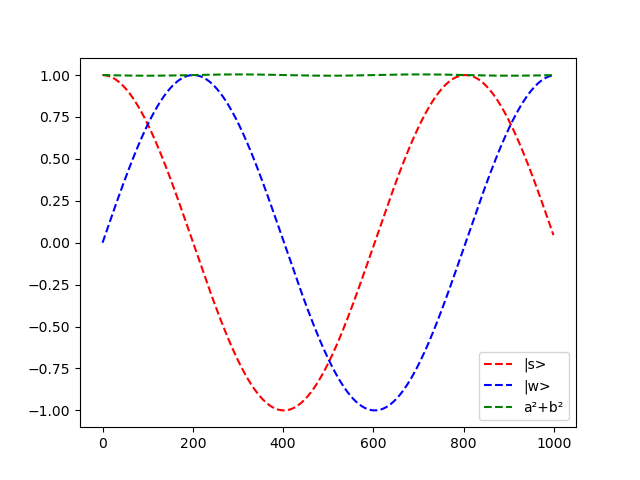
\includegraphics[scale=0.6]{Grover/grover_n16_1000.png}
  \caption{Evolution des amplitudes pour n=16, sur 1000 itérations}
  \label{fig:univerise}
\end{figure}

\subsection{Implémentation}

\subsubsection*{Simulation sur un ordinateur classique}

% \begin{lstlisting}[language=Python]
% import numpy as np
% import math
% import random

% N = 2**8
% n_opti = (math.pi/4)*math.sqrt(N)
% nb_iter = math.floor(n_opti)
% w = np.zeros((N, 1))
% w[random.randint(-1, N)] = np.imag(0 + 1j)
% s = np.ones((N, 1)) / math.sqrt(N)
% u_w = np.identity(N) - 2 * w * np.transpose(w)
% u_s = 2 * s * np.transpose(s) - np.identity(N)
% g = np.dot(u_s, u_w)
% x = s
% for i in range(0, nb_iter):
%     x = np.dot(g, x)
% \end{lstlisting}

\begin{algorithm}[H]
  \SetAlgoLined
  \KwData{
    $w$ vector of size $2^n$ of $0$ with target index to 1;
  }

  \KwOut{
    $x$ vector of amplitudes (largest amplitude corresponding to wanted index)
  }

  \Begin{
    $s$ vector of size $2^n$ of $\frac{1}{\sqrt{2^n}}$
    $N \longleftarrow 2^n$\;
    $N_{iter} \longleftarrow floor(\frac{\pi}{4} \sqrt{N})$\;
    \tcc{Compute grover operator}
    $U_w \longleftarrow I_N - 2 w \cdot w^T$\;
    $U_s \longleftarrow 2 s \cdot s^T - I_N$\;
    $g \longleftarrow U_s \cdot U_w$\;
    $x \longleftarrow s$ \;
    \tcc{Apply grover operator $N_{iter}$ times}
    \For(){$i = 0$ \KwTo $N_{iter}$}{
      $x \longleftarrow g \cdot x $\;
    }
  }
\end{algorithm}

% \subsubsection*{Algorithme quantique}

% \begin{lstlisting}[language=Python]
% import numpy as np
% import math
% import random
% from qiskit import QuantumRegister, ClassicalRegister, QuantumCircuit

% var_qubits = QuantumRegister(4, name='v')
% clause_qubits = QuantumRegister(4, name='c')
% output_qubits = QuantumRegister(1, name='out')
% cbits = ClassicalRegister(4, name='cbits')
% qc = QuantumCircuit(var_qubits, clause_qubits, output_qubits, cbits)
% qc.initialize([1, -1]/np.sqrt(2), output_qubits)
% qc.h(var_qubits)
% qc.barrier()

% \end{lstlisting}